\documentclass[12pt]{article}

\usepackage[a4paper,margin=1in]{geometry}
\usepackage[T1]{fontenc}
\usepackage[utf8]{inputenc}
\usepackage{graphicx}
\usepackage{hyperref}
\usepackage{booktabs}
\usepackage{array}
\usepackage{tabularx}
\usepackage{float}
\usepackage{setspace}
\usepackage{caption}
\usepackage{xcolor}
\usepackage{url}

\hypersetup{
    colorlinks=true,
    linkcolor=blue,
    urlcolor=blue,
    citecolor=blue
}

\setlength{\parindent}{0pt}
\setlength{\parskip}{0.55em}
\onehalfspacing
\captionsetup{font=small,skip=4pt}
\newcolumntype{Y}{>{\raggedright\arraybackslash}X}

\title{Learning-Enhanced Personnel Scheduling for Flexible Multi-Skilled Workforces\\Abridged Literature Review}
\author{Mingyuan Liu \\ Student ID: 20808220}
\date{}

\begin{document}
\emergencystretch=1.5em

\maketitle

\section{Introduction and Motivation}

Personnel scheduling is central to retail, hospitality, healthcare, and other service settings where demand changes over time and employees differ in skills, contracts, and preferences. Although the field has been studied extensively in operations research, real-world adoption remains limited because classical models often capture feasibility and cost more effectively than tacit human preferences or operational nuance \cite{ernst2004,vandenbergh2013,petrovic2017}. This abridged review examines 17 papers from 2004 to 2025. Anchored on Xue et al.\ (2025), it positions flexible, multi-skilled, learning-enhanced scheduling as a response to that adoption gap \cite{xue2025}. The field now moves beyond feasibility and cost, yet still struggles to encode managerial preferences without losing tractability.

\begin{figure}[H]
\centering
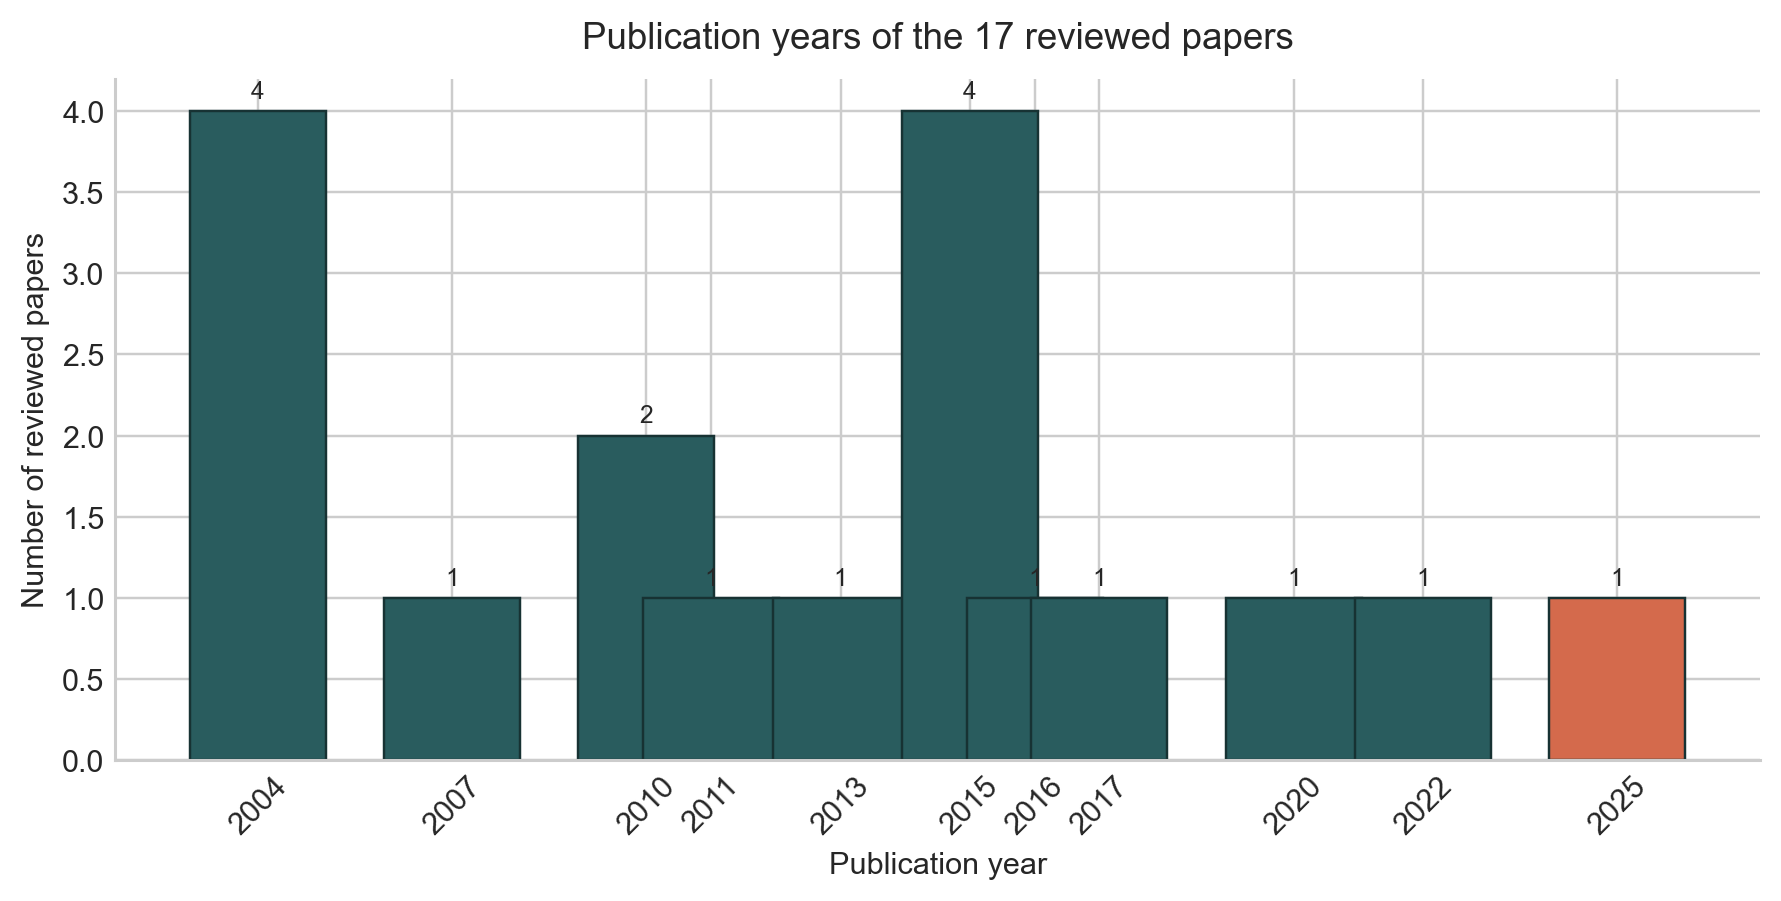
\includegraphics[width=0.72\textwidth]{figures/publication_year_histogram.png}
\caption{Publication years of the 17 reviewed papers. The concentration after 2010 suggests growing interest in flexible, skill-aware, and implementation-oriented personnel scheduling.}
\label{fig:histogram}
\end{figure}

\subsection{Research Field Challenges}

Four challenges dominate. First, \textit{scalability} worsens when flexible shifts enlarge the search space combinatorially \cite{xue2025}. Second, \textit{heterogeneity} matters because skills, contracts, and availability create interdependent assignment constraints that homogeneous formulations cannot capture well \cite{debruecker2015,hojati2011}. Third, \textit{demand uncertainty} creates mismatch between staffing plans and realised service needs in service environments \cite{defraeye2016,parisio2015}. Fourth, a persistent \textit{research-practice gap} means strong objective values do not guarantee adoption if schedules violate tacit rules or fairness expectations \cite{petrovic2017}. Personnel scheduling is therefore a decision-support problem as well as an assignment problem.

\section{Methodology}

\subsection{Search Strategy}

The search began with Xue et al.\ (2025) as the seed paper. Related work was expanded through ConnectedPapers, backward citation chasing, and searches in ScienceDirect, SpringerLink, IEEE Xplore, and Google Scholar. Core keywords included ``personnel scheduling'', ``staff rostering'', ``flexible shift scheduling'', ``multi-skilled workforce scheduling'', ``shift design'', ``shift assignment'', ``preference-aware scheduling'', and ``learning-enhanced optimisation''. The final set was narrowed to papers directly relevant to flexible shifts, workforce heterogeneity, implementation, or machine-learning-assisted optimisation.

\begin{figure}[H]
\centering
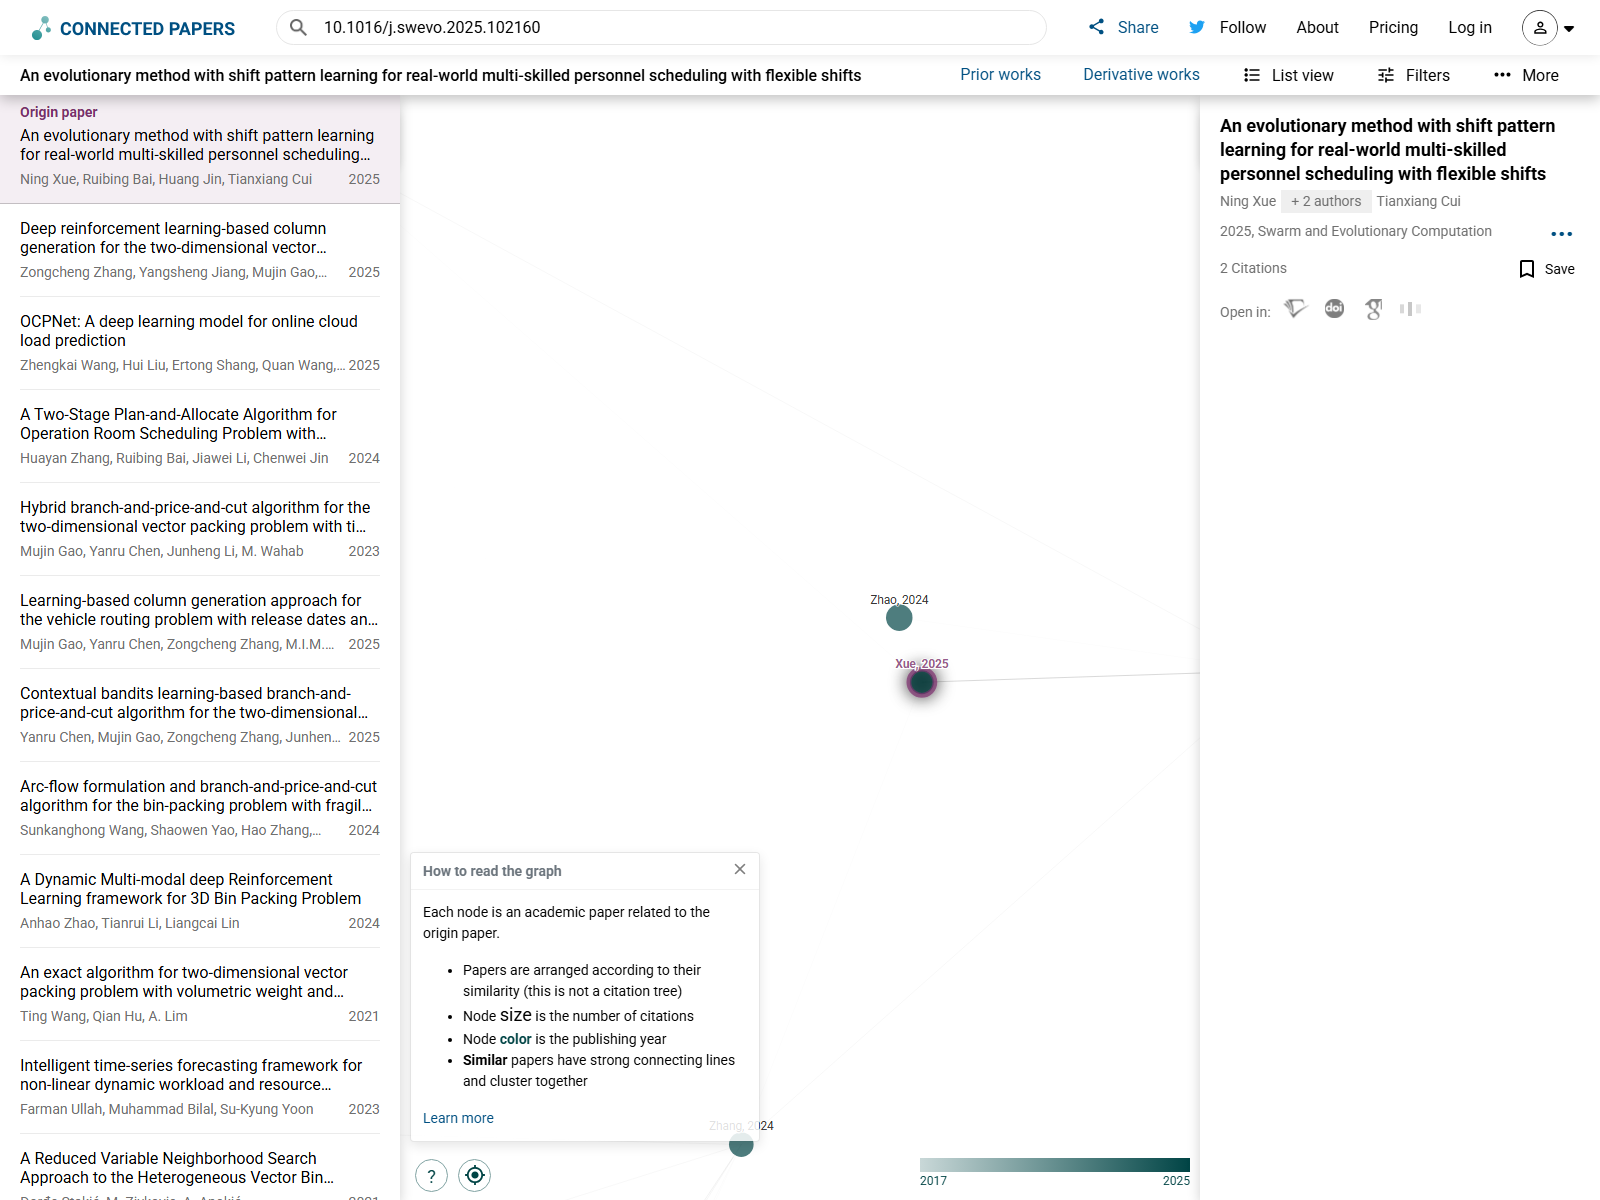
\includegraphics[width=0.82\textwidth]{figures/connectedpapers_graph.png}
\caption{ConnectedPapers graph illustrating citation-based expansion from the seed paper by Xue et al.\ (2025).}
\label{fig:connectedpapers}
\end{figure}

\subsection{Survey Scope}

The review includes peer-reviewed papers published between 2004 and 2025 with identifiable DOIs and a clear connection to personnel scheduling, workforce scheduling, or staff rostering. Survey papers were retained when they define the field or classify major modelling choices. Papers were excluded if they focused on routing without workforce scheduling, general HR policy, or lacked a usable DOI. This scope keeps the review close to learning-enhanced scheduling for flexible, multi-skilled workforces.

\subsection{Article Statistical Analysis}

The search yielded 42 candidate papers. After removing 21 papers for relevance or DOI issues, 26 papers were screened at full-text level and 17 were retained.

\begin{table}[H]
\centering
\caption{Article screening summary}
\label{tab:screening}
\begin{tabular}{lr}
\toprule
Stage & Count \\
\midrule
Seed paper & 1 \\
ConnectedPapers and database candidates & 42 \\
Removed after relevance / DOI screening & 21 \\
Full-text papers screened & 26 \\
Final papers included & 17 \\
\bottomrule
\end{tabular}
\end{table}

\section{Classification of Literature}

The papers are organised by their main contribution: defining the field, addressing implementation and preferences, structuring flexible-shift design, or improving optimisation with hybrid and learning-enhanced methods.

\begin{table}[H]
\centering
\caption{Classification scheme for the reviewed literature}
\label{tab:classification}
\small
\begin{tabularx}{\textwidth}{p{0.17\textwidth}p{0.27\textwidth}Y}
\toprule
Category & Main focus & Papers \\
\midrule
A. Surveys and field framing & Field definitions, skill planning, demand uncertainty & Ernst et al.\ (2004); Van den Bergh et al.\ (2013); De Bruecker et al.\ (2015); Defraeye and Van Nieuwenhuyse (2016) \\
B. Preference and implementation & Human preferences, deployment, industry cases & Gordon and Erkut (2004); Topaloglu and Ozkarahan (2004); Henao et al.\ (2015); Petrovic (2017) \\
C. Shift design and decomposition & Shift construction, part-time staffing, uncertainty & Di Gaspero et al.\ (2007); Hojati and Patil (2011); Parisio and Jones (2015); Prot et al.\ (2015) \\
D. Evolutionary and learning-enhanced methods & Evolutionary baselines, matheuristics, ML-guided search & Aickelin and Dowsland (2004); Bai et al.\ (2010); \c{C}ak{\i}rgil et al.\ (2020); Sun et al.\ (2022); Xue et al.\ (2025) \\
\bottomrule
\end{tabularx}
\end{table}

\begin{figure}[H]
\centering
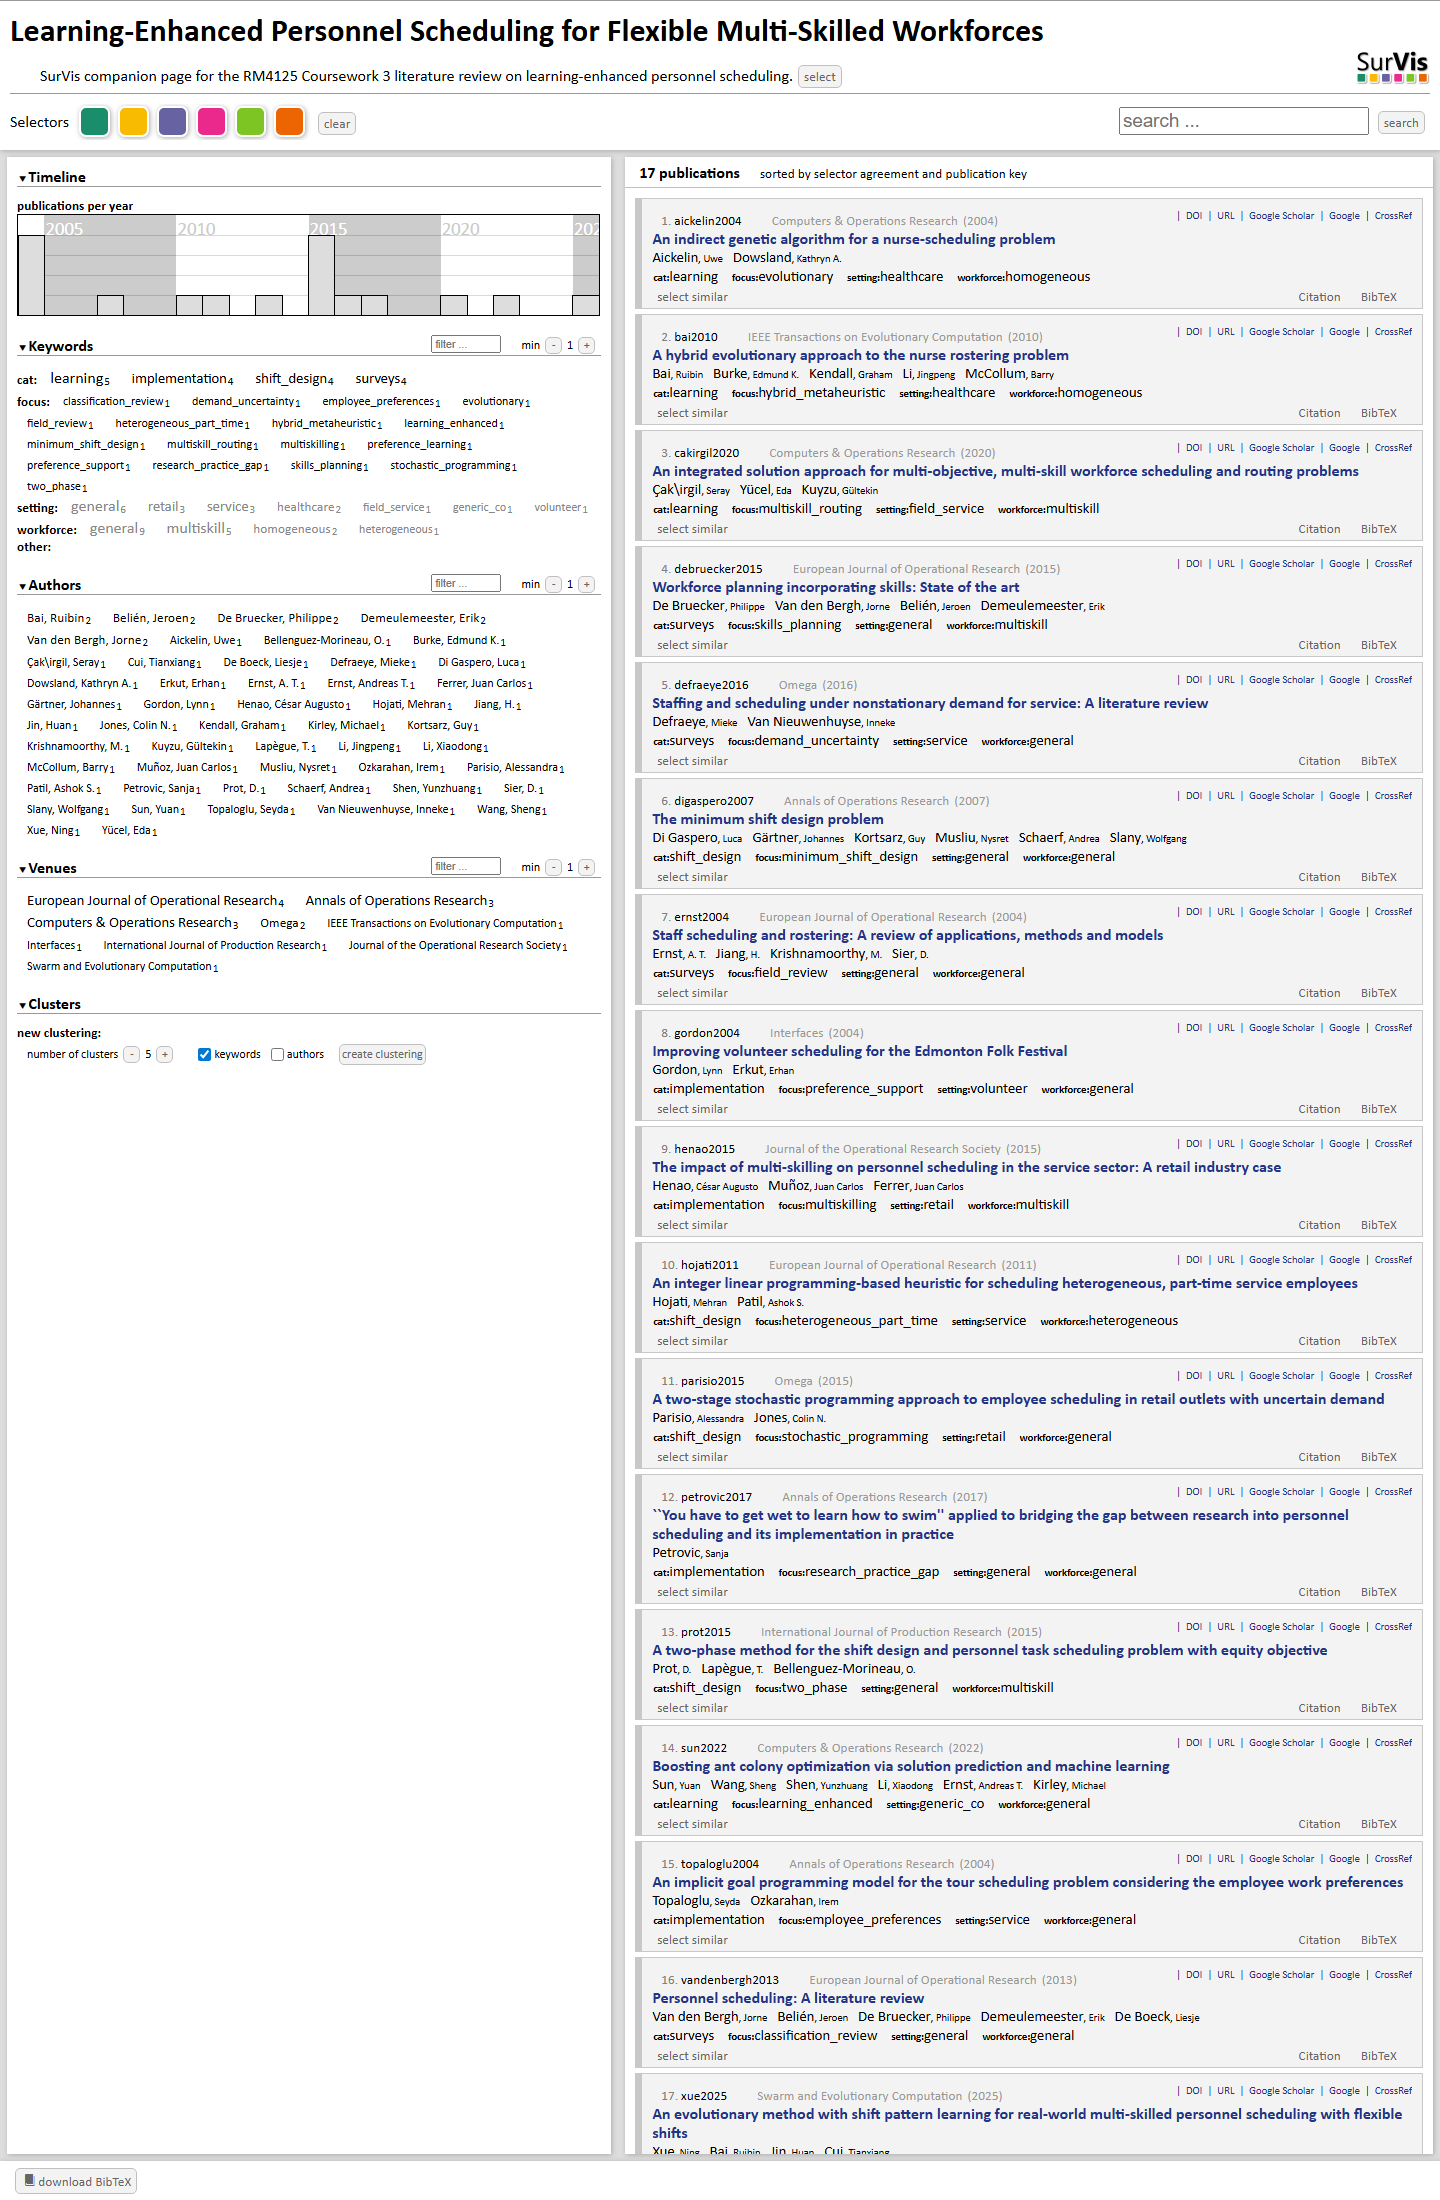
\includegraphics[width=0.82\textwidth]{figures/figure_survis_screenshot.png}
\caption{SurVis companion page generated from the 17-paper bibliography, showing the timeline, tag filters, and searchable entry list used to support the classification.}
\label{fig:survis}
\end{figure}

\textbf{SurVis public URL:}\\
\url{https://lmy12367.github.io/learning-enhanced-scheduling-survis/}

\subsection{Category A: Surveys and Field Framing}

\textbf{Ernst et al.\ (2004).} This foundational review synthesises applications, models, and solution methods across staff scheduling and rostering. It does not propose a new algorithm; instead, it clarifies how objectives and constraints vary by application domain. That broad framing still anchors contemporary scheduling research \cite{ernst2004}.

\textbf{Van den Bergh et al.\ (2013).} This review classifies personnel scheduling literature from multiple perspectives, including problem setting and technical features. Its table-based structure is especially useful for identifying research trends and neglected combinations of characteristics. It therefore serves as a practical survey seed for the present review \cite{vandenbergh2013}.

\textbf{De Bruecker et al.\ (2015).} This state-of-the-art review focuses on workforce planning with skill considerations. By moving beyond single-skill staffing, it helps explain why multi-skilled personnel scheduling cannot be treated as a minor extension of standard rostering. The paper broadens the conceptual basis for skill-aware scheduling \cite{debruecker2015}.

\textbf{Defraeye and Van Nieuwenhuyse (2016).} This literature review examines staffing and scheduling under nonstationary demand in service systems. Its main relevance is to show that fluctuating demand is not a peripheral complication but a central modelling driver. That insight links classical service operations research to flexible workforce scheduling \cite{defraeye2016}.

These surveys map the problem space well, but they do not explain how preferences or deployment realities should enter operational models.

\subsection{Category B: Preference and Implementation}

\textbf{Gordon and Erkut (2004).} Gordon and Erkut describe a spreadsheet-based decision-support tool for volunteer scheduling at the Edmonton Folk Festival. The work is important because it addresses implementation, user preferences, and usable schedule outputs rather than only optimisation quality. It shows how adoption concerns can dominate model choice in practice \cite{gordon2004}.

\textbf{Topaloglu and Ozkarahan (2004).} This paper presents an implicit goal programming model for tour scheduling that incorporates employee work preferences and scheduling flexibility. The integrated formulation generates work schedules without a separate downstream assignment step. It is an early example of preference-aware scheduling as a primary modelling objective \cite{topaloglu2004}.

\textbf{Henao et al.\ (2015).} Henao et al.\ study multi-skilling in a retail service case through a mixed-integer model for training and assignment decisions over a weekly horizon. Their results suggest that selective, not universal, multi-skilling can improve schedule efficiency. The paper is especially relevant because it ties personnel flexibility to a concrete retail setting \cite{henao2015}.

\textbf{Petrovic (2017).} Petrovic offers a critical reflection on why personnel scheduling research still has limited practical uptake. By classifying existing software and discussing what schedulers actually need, the paper reframes implementation as a research problem in its own right. It is central for understanding the gap between theoretical optimisation and deployed systems \cite{petrovic2017}.

These studies confront adoption more directly, but most still rely on conventional optimisation rather than learned representations of human judgement.

\subsection{Category C: Shift Design and Decomposition}

\textbf{Di Gaspero et al.\ (2007).} This paper studies the minimum shift design problem and connects it to a network-flow formulation. It proposes a hybrid heuristic combining greedy construction with local search, and experiments show clear gains over an earlier implementation. The paper is valuable because it isolates shift design as a standalone analytical task \cite{digaspero2007}.

\textbf{Hojati and Patil (2011).} Hojati and Patil address the scheduling of heterogeneous, part-time service employees using an integer linear programming-based heuristic. The paper is relevant because it models precisely the kind of mixed-skill and part-time labour structure that later flexible workforce studies inherit. It therefore bridges service scheduling and heterogeneous workforce assignment \cite{hojati2011}.

\textbf{Parisio and Jones (2015).} Parisio and Jones formulate employee scheduling in retail outlets as a two-stage stochastic programming problem with uncertain demand. Their contribution is to embed demand uncertainty directly into workforce planning rather than treating it as an afterthought. This makes the paper important for real-world retail settings with volatile service loads \cite{parisio2015}.

\textbf{Prot et al.\ (2015).} Prot et al.\ propose a two-phase method for the shift design and personnel task scheduling problem with an equity objective. By iterating between design and assignment, the paper shows that decomposed methods can remain coordinated rather than naively sequential. Its structure closely foreshadows the two-stage logic used in later flexible scheduling research \cite{prot2015}.

Category C increases realism through decomposition and uncertainty handling, but usually at the cost of globally integrated optimisation.

\subsection{Category D: Evolutionary and Learning-Enhanced Methods}

\textbf{Aickelin and Dowsland (2004).} This paper develops an indirect genetic algorithm for nurse scheduling using permutation encoding and a heuristic decoder. Computational experiments on live hospital data show that the approach is flexible, fast, and competitive with tabu search. It remains a useful baseline for later evolutionary scheduling work \cite{aickelin2004}.

\textbf{Bai et al.\ (2010).} Bai et al.\ improve nurse rostering by hybridising stochastic-ranking genetic search with a simulated-annealing hyper-heuristic. Their experiments show better feasible and high-quality solutions than earlier evolutionary baselines. The paper is significant because it demonstrates how hybrid search can outperform single-technique metaheuristics \cite{bai2010}.

\textbf{\c{C}ak{\i}rgil et al.\ (2020).} This study examines multi-objective, multi-skill workforce scheduling and routing for field service operations. It combines a mixed-integer model with a two-stage matheuristic and validates the approach on real-life and literature instances. The paper expands the review beyond rostering to richer service operations with team formation and routing \cite{cakirgil2020}.

\textbf{Sun et al.\ (2022).} Sun et al.\ propose ML-ACO, where a learned predictor estimates promising solution components before ant colony optimisation constructs routes. The paper is not about personnel scheduling directly, but it offers a transferable template for integrating supervised learning into metaheuristic search. It therefore supports the broader move toward learning-enhanced optimisation \cite{sun2022}.

\textbf{Xue et al.\ (2025).} Xue et al.\ address real-world personnel scheduling with flexible shifts and multi-skilled part-time workers through a machine-learning-enhanced memetic algorithm. A decision tree learns appealing historical shift patterns, while a two-phase framework separates shift design from assignment. This paper is the anchor study because it directly combines practical realism, preference learning, and advanced search \cite{xue2025}.

Category D strengthens search performance, yet most methods still depend on handcrafted encodings; Xue et al.\ (2025) is distinctive in learning from historical scheduling patterns.

\section{Discussion}

A key insight from the reviewed literature is that the main bottleneck is no longer pure computational optimisation but model realism. Early work emphasised how to solve difficult schedules, whereas recent studies argue that deployment fails when models omit tacit preferences, flexibility, or contextual constraints \cite{petrovic2017,xue2025}. There is therefore a clear tension between realism and tractability: flexible shifts, heterogeneous skills, and uncertain demand improve fidelity, but they also push researchers toward decomposition, heuristics, or matheuristics \cite{digaspero2007,parisio2015,prot2015}. No reviewed study fully integrates flexible shift design, multi-skilled workforce modelling, data-driven preference learning, and real-world deployment validation in one tested framework. Public benchmarks remain limited, and learned components are rarely evaluated for transferability or bias. Figure~\ref{fig:framework} summarises this review's synthesis of the field.

\begin{figure}[H]
\centering
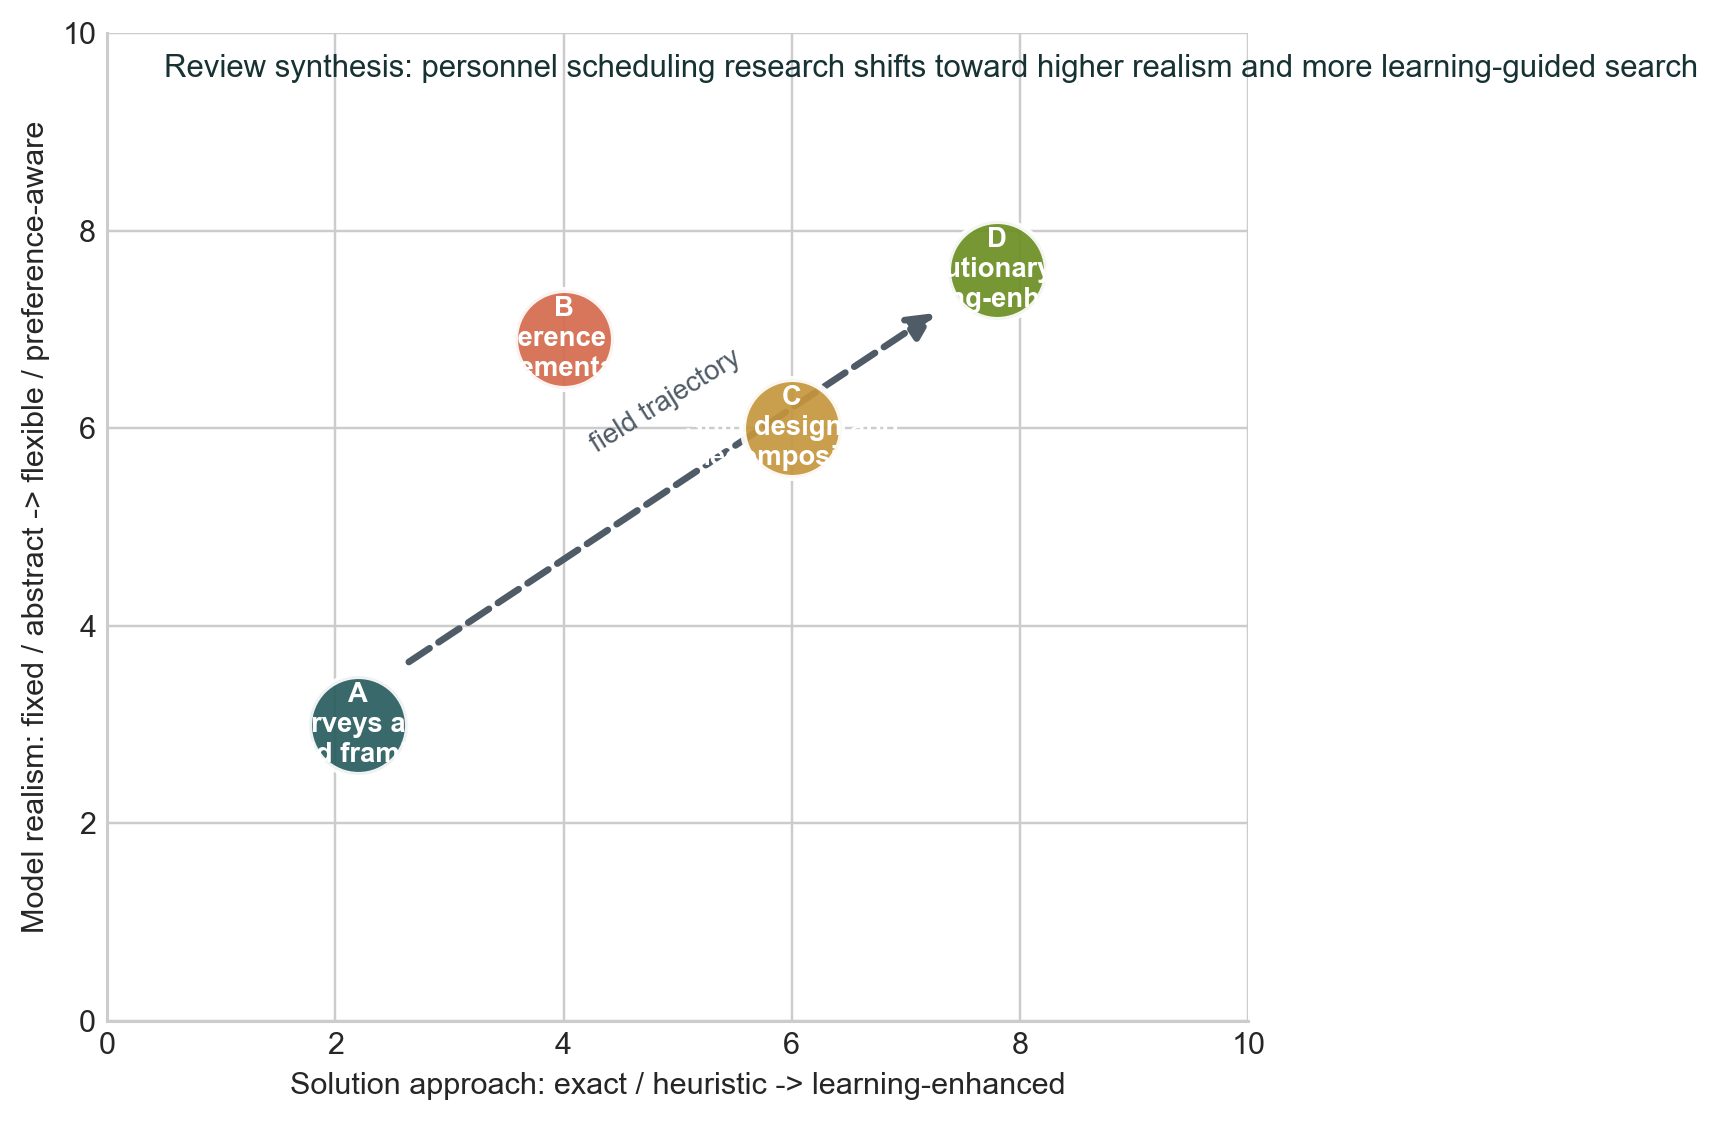
\includegraphics[width=0.74\textwidth]{figures/figure_conceptual_framework.png}
\caption{Conceptual framework synthesised from the review. Most studies cluster in intermediate regions; very few combine high model realism with learning-enhanced optimisation.}
\label{fig:framework}
\end{figure}

\section{Conclusion}

This review shows that personnel scheduling research is moving from generic rostering toward flexible, skill-aware decision support. Survey papers define the field, implementation papers explain adoption barriers, and newer hybrid methods point toward more realistic optimisation. A promising dissertation direction is interpretable learning-enhanced personnel scheduling under demand volatility and workforce heterogeneity.

\renewcommand{\refname}{References}
\begin{thebibliography}{99}

\bibitem{aickelin2004}
Aickelin, U., \& Dowsland, K. A. (2004).
An indirect genetic algorithm for a nurse-scheduling problem.
\textit{Computers \& Operations Research, 31}(5), 761--778.
\url{https://doi.org/10.1016/S0305-0548(03)00034-0}

\bibitem{bai2010}
Bai, R., Burke, E. K., Kendall, G., Li, J., \& McCollum, B. (2010).
A hybrid evolutionary approach to the nurse rostering problem.
\textit{IEEE Transactions on Evolutionary Computation, 14}(4), 580--590.
\url{https://doi.org/10.1109/TEVC.2009.2033583}

\bibitem{cakirgil2020}
\c{C}ak{\i}rgil, S., Y\"ucel, E., \& Kuyzu, G. (2020).
An integrated solution approach for multi-objective, multi-skill workforce scheduling and routing problems.
\textit{Computers \& Operations Research, 118}, 104908.
\url{https://doi.org/10.1016/j.cor.2020.104908}

\bibitem{debruecker2015}
De Bruecker, P., Van den Bergh, J., Beli\'en, J., \& Demeulemeester, E. (2015).
Workforce planning incorporating skills: State of the art.
\textit{European Journal of Operational Research, 243}(1), 1--16.
\url{https://doi.org/10.1016/j.ejor.2014.10.038}

\bibitem{defraeye2016}
Defraeye, M., \& Van Nieuwenhuyse, I. (2016).
Staffing and scheduling under nonstationary demand for service: A literature review.
\textit{Omega, 58}, 4--25.
\url{https://doi.org/10.1016/j.omega.2015.04.002}

\bibitem{digaspero2007}
Di Gaspero, L., G\"artner, J., Kortsarz, G., Musliu, N., Schaerf, A., \& Slany, W. (2007).
The minimum shift design problem.
\textit{Annals of Operations Research, 155}(1), 79--105.
\url{https://doi.org/10.1007/s10479-007-0221-1}

\bibitem{ernst2004}
Ernst, A. T., Jiang, H., Krishnamoorthy, M., \& Sier, D. (2004).
Staff scheduling and rostering: A review of applications, methods and models.
\textit{European Journal of Operational Research, 153}(1), 3--27.
\url{https://doi.org/10.1016/S0377-2217(03)00095-X}

\bibitem{gordon2004}
Gordon, L., \& Erkut, E. (2004).
Improving volunteer scheduling for the Edmonton Folk Festival.
\textit{Interfaces, 34}(5), 367--376.
\url{https://doi.org/10.1287/inte.1040.0097}

\bibitem{henao2015}
Henao, C. A., Mu\~noz, J. C., \& Ferrer, J. C. (2015).
The impact of multi-skilling on personnel scheduling in the service sector: A retail industry case.
\textit{Journal of the Operational Research Society, 66}(12), 1949--1959.
\url{https://doi.org/10.1057/jors.2015.9}

\bibitem{hojati2011}
Hojati, M., \& Patil, A. S. (2011).
An integer linear programming-based heuristic for scheduling heterogeneous, part-time service employees.
\textit{European Journal of Operational Research, 209}(1), 37--50.
\url{https://doi.org/10.1016/j.ejor.2010.09.004}

\bibitem{parisio2015}
Parisio, A., \& Jones, C. N. (2015).
A two-stage stochastic programming approach to employee scheduling in retail outlets with uncertain demand.
\textit{Omega, 53}, 97--103.
\url{https://doi.org/10.1016/j.omega.2015.01.003}

\bibitem{petrovic2017}
Petrovic, S. (2017).
``You have to get wet to learn how to swim'' applied to bridging the gap between research into personnel scheduling and its implementation in practice.
\textit{Annals of Operations Research, 275}(1), 161--179.
\url{https://doi.org/10.1007/s10479-017-2574-4}

\bibitem{prot2015}
Prot, D., Lap\`egue, T., \& Bellenguez-Morineau, O. (2015).
A two-phase method for the shift design and personnel task scheduling problem with equity objective.
\textit{International Journal of Production Research, 53}(24), 7286--7298.
\url{https://doi.org/10.1080/00207543.2015.1037023}

\bibitem{sun2022}
Sun, Y., Wang, S., Shen, Y., Li, X., Ernst, A. T., \& Kirley, M. (2022).
Boosting ant colony optimization via solution prediction and machine learning.
\textit{Computers \& Operations Research, 143}, 105769.
\url{https://doi.org/10.1016/j.cor.2022.105769}

\bibitem{topaloglu2004}
Topaloglu, S., \& Ozkarahan, I. (2004).
An implicit goal programming model for the tour scheduling problem considering the employee work preferences.
\textit{Annals of Operations Research, 128}(1--4), 135--158.
\url{https://doi.org/10.1023/B:ANOR.0000019102.68222.df}

\bibitem{vandenbergh2013}
Van den Bergh, J., Beli\'en, J., De Bruecker, P., Demeulemeester, E., \& De Boeck, L. (2013).
Personnel scheduling: A literature review.
\textit{European Journal of Operational Research, 226}(3), 367--385.
\url{https://doi.org/10.1016/j.ejor.2012.11.029}

\bibitem{xue2025}
Xue, N., Bai, R., Jin, H., \& Cui, T. (2025).
An evolutionary method with shift pattern learning for real-world multi-skilled personnel scheduling with flexible shifts.
\textit{Swarm and Evolutionary Computation, 99}, 102160.
\url{https://doi.org/10.1016/j.swevo.2025.102160}

\end{thebibliography}

\end{document}
